\documentclass{beamer}
\usepackage[utf8]{inputenc}

% Use UTCS theme:
\usetheme[]{utcs}

\usepackage[]{graphicx}
\usepackage[]{color}

\usepackage{accents}

\usepackage{subcaption}
\usepackage{tikz}
\usetikzlibrary{calc}
\usepackage[export]{adjustbox}
% externalize tikz
\usetikzlibrary{external}
\tikzexternalize[prefix=./tikz/]

\usepackage{amssymb,latexsym,amsmath}
\usepackage{amsfonts}
\usepackage{amsbsy}

\usepackage{minted}

\newcommand{\sep}{\setlength\arraycolsep{2pt}}
\def\disp{\displaystyle}

\author[BMS]{Robert Kirby$^{1}$
\and Andreas Kl\"ockner$^{2}$
\and Ben Sepanski$^{3}$
}
\date{25 March 2021}
\institute{$^{1}$Baylor University
\\ $^{2}$University of Illinois at Urbana-Champaign
\\ $^{3}$University of Texas at Austin
}
\title{Nonlocal UFL:\@ Finite elements for Helmholtz equations with a nonlocal boundary condition}
\logo{
\includegraphics[width=1.5cm]{figs/cslogo.eps}}

\begin{document}

%%%%%%%%%%%%%%%%%%%%%%%%             %%%%%%%%%%%%%%%%%%%%%%%%
%%%%%%%%%%%%%%%%%%%%%%%  Title frame  %%%%%%%%%%%%%%%%%%%%%%%%
%%%%%%%%%%%%%%%%%%%%%%%%             %%%%%%%%%%%%%%%%%%%%%%%%
\begin{frame}[noframenumbering]
    \titlepage
\end{frame}

%%%%%%%%%%%%%%%%%%%%%%%%     %%%%%%%%%%%%%%%%%%%%%%%%
%%%%%%%%%%%%%%%%%%%%%%%  TOC  %%%%%%%%%%%%%%%%%%%%%%%%
%%%%%%%%%%%%%%%%%%%%%%%%     %%%%%%%%%%%%%%%%%%%%%%%%
\begin{frame}[noframenumbering]{Order of Presentation}
    \tableofcontents
\end{frame}

\begin{frame}[noframenumbering]
\frametitle{Thanks to\ldots}
\begin{block}{}
\begin{itemize}
\item NSF 1525697, 1909176
\item The U.S. Department of Energy, Office of
Science, Office of Advanced Scientific Computing
Research, Department of Energy Computational Science
Graduate Fellowship under Award Number DE-SC0021110
\item Luke Olson (UIUC)
\end{itemize}
\end{block}
\end{frame}

%%%%%%%%%%%%%%%%%%%%%%%%                             %%%%%%%%%%%%%%%%%%%%%%%%
%%%%%%%%%%%%%%%%%%%%%%%  SECTION: Motivating problem  %%%%%%%%%%%%%%%%%%%%%%%%
%%%%%%%%%%%%%%%%%%%%%%%%                             %%%%%%%%%%%%%%%%%%%%%%%%
\section{Motivating Problem: Helmholtz scattering}

% slide numbers
\setbeamertemplate{footline}[frame number]

%%%%%%%%%%%%%%%%%%%%%%%%                             %%%%%%%%%%%%%%%%%%%%%%%%
%%%%%%%%%%%%%%%%%%%%%%%  Helmholtz radiation problem  %%%%%%%%%%%%%%%%%%%%%%%%
%%%%%%%%%%%%%%%%%%%%%%%%                             %%%%%%%%%%%%%%%%%%%%%%%%
\begin{frame}{Exterior scattering}
    \begin{columns}
    \begin{column}{0.45\textwidth}
        \begin{figure}[ht]
        \begin{center}
        \begin{tikzpicture}[scale=0.8]
            \draw [thick,fill=black!30] (-3,-3) rectangle (3,3)
            (0, 0) circle (1);
            \node at (0,0) {$\Omega^c$};
            \node at (-2,2) {$\Omega'$};
            \node [anchor=west] at (1,0) {$\Gamma$};
            \node [anchor=west] at (3,0) {$\Sigma$};
        \end{tikzpicture}
        \end{center}\label{fig:2ddomain}
        \end{figure}
    \end{column}
    \begin{column}{0.55\textwidth}
        \begin{itemize}
            \item<1-> Model waves reflecting off of obstacle $\Gamma$
            \[
                \begin{cases}
                    -\Delta u + \kappa^2 u = 0, &  \mathbb R^d\setminus\Omega \\
                    -\frac{\partial u}{\partial n} = f, & \Gamma
                \end{cases}
            \]
            \item<2-> \emph{Without} any spurious reflections from infinity
            \[
                \lim_{r\to\infty} r^{(d-1)/2}
                    \left(\tfrac{\partial u}{\partial r} - i\kappa u\right)
                = 0
            \]
            \item<3-> In some finite domain of interest 
            $\Omega'\subseteq \mathbb R^d\setminus\Omega'$
            bounded by $\Sigma$.
        \end{itemize}
    \end{column}
\end{columns}
\end{frame}

%%%%%%%%%%%%%%%%%%%%%%%%                   %%%%%%%%%%%%%%%%%%%%%%%%
%%%%%%%%%%%%%%%%%%%%%%%  But what are BCs?  %%%%%%%%%%%%%%%%%%%%%%%%
%%%%%%%%%%%%%%%%%%%%%%%%                   %%%%%%%%%%%%%%%%%%%%%%%%
\begin{frame}{Exterior scattering: computational problem}
    \begin{columns}
    \begin{column}{0.45\textwidth}
        \begin{figure}[ht]
        \begin{center}
        \begin{tikzpicture}[scale=0.8]
            \draw [thick,fill=black!30] (-3,-3) rectangle (3,3)
            (0, 0) circle (1);
            \node at (0,0) {$\Omega^c$};
            \node at (-2,2) {$\Omega'$};
            \node [anchor=west] at (1,0) {$\Gamma$};
            \node [anchor=west] at (3,0) {$\Sigma$};
        \end{tikzpicture}
        \end{center}
        \end{figure}
    \end{column}
    \begin{column}{0.55\textwidth}
        \begin{itemize}
            \item<1-> Problem we want to solve
            \[
                \begin{cases}
                    -\Delta u + \kappa^2 u = 0, &  \mathbb R^d\setminus\Omega \\
                    -\frac{\partial u}{\partial n} = f, & \Gamma \\
                    \lim_{r\to\infty} r^{(d-1)/2}
                        \left(\tfrac{\partial u}{\partial r} - i\kappa u\right)
                = 0
                \end{cases}
            \]
            \item<2-> Problem we can actually solve
            \[
                \begin{cases}
                    -\Delta u + \kappa^2 u = 0, & \Omega' \\
                    -\frac{\partial u}{\partial n} = f, & \Gamma \\
                    ?????, & \Sigma
                \end{cases}
            \]
        \end{itemize}
    \end{column}
    \end{columns}
\end{frame}


%%%%%%%%%%%%%%%%%%%%%%%%              %%%%%%%%%%%%%%%%%%%%%%%%
%%%%%%%%%%%%%%%%%%%%%%%  PML Approach  %%%%%%%%%%%%%%%%%%%%%%%%
%%%%%%%%%%%%%%%%%%%%%%%%              %%%%%%%%%%%%%%%%%%%%%%%%
\begin{frame}{Exterior scattering: PML}
    \begin{columns}
    \begin{column}{0.45\textwidth}
        \begin{figure}[ht]
        \begin{center}
        \begin{tikzpicture}[scale=0.8]
            \draw [thick,fill=black!30] (-3,-3) rectangle (3,3)
            (0, 0) circle (1);
            \node at (0,0) {$\Omega^c$};
            \node at (-2,2) {$\Omega'$};
            \node [anchor=west] at (1,0) {$\Gamma$};
            \node [anchor=west] at (3,0) {$\Sigma$};
        \end{tikzpicture}
        \end{center}
        \end{figure}
    \end{column}
    \begin{column}{0.55\textwidth}
        \begin{itemize}
            \item Perfectly Matched Layers:
            \[
                \begin{cases}
                    -\nabla \cdot \beta(x) \nabla u + \kappa^2 u = 0,  & \Omega^\prime \\
                    -\frac{\partial u}{\partial n}  =  f, &\Gamma \\
                    u = 0, &\Sigma
                \end{cases}
            \]
              \item<2-> $\beta = I$ in $\Omega^\prime$
              \item<3-> $\beta$ is complex-valued, eats waves in $\Omega_S$
              \item<4-> Solution is right in $\Omega^\prime$
              \item<5-> {\bf Solvers are a pain!}
        \end{itemize}
    \end{column}
    \end{columns}
\end{frame}

%%%%%%%%%%%%%%%%%%%%%%%%                           %%%%%%%%%%%%%%%%%%%%%%%%
%%%%%%%%%%%%%%%%%%%%%%%  Integral equations review  %%%%%%%%%%%%%%%%%%%%%%%%
%%%%%%%%%%%%%%%%%%%%%%%%                           %%%%%%%%%%%%%%%%%%%%%%%%
\section{A nonlocal boundary condition}

\begin{frame}{Integral form of the solution}
With $\mathcal{K}$ the Green's function, the \emph{true} solution satisfies:
  \begin{equation*}
      u(x) = D(u)(x) - S(\tfrac{\partial}{\partial n})(x), \quad x \in\Omega'
  \end{equation*}
  where
\visible<2->{
    \begin{equation*}
        D(u)(x) = \int_\Gamma \left( \tfrac{\partial}{\partial n} \mathcal K( x-y) \right)u(y) dy, 
    \end{equation*}
}
\visible<3->{
    \begin{equation*}
    S(u)(x) = \int  \mathcal K (x - y ) u(y)dy
    \end{equation*}
}
\end{frame}

%%%%%%%%%%%%%%%%%%%%%%%        %%%%%%%%%%%%%%%%%%%%%%%%
%%%%%%%%%%%%%%%%%%%%%%  Our BC  %%%%%%%%%%%%%%%%%%%%%%%%
%%%%%%%%%%%%%%%%%%%%%%%        %%%%%%%%%%%%%%%%%%%%%%%%
\begin{frame}{Exterior scattering}
  \begin{columns}
    \begin{column}{0.35\textwidth}
    \begin{figure}[ht]
        \begin{center}
        \begin{tikzpicture}[scale=0.4]
          \draw [thick,fill=black!30] (-3,-3) rectangle (3,3)
            (0, 0) circle (1);
          \node at (0,0) {$\Omega^c$};
          \node at (-2,2) {$\Omega'$};
          \node [anchor=west] at (1,0) {$\Gamma$};
          \node [anchor=west] at (3,0) {$\Sigma$};
        \end{tikzpicture}
        \end{center}
        %\caption{A 2D example of a truncated domain}
        %\label{fig:2ddomain}
      \end{figure}
        \end{column}
        \begin{column}{0.65\textwidth}
                \emph{Exact} boundary conditions
                 \[
                     \begin{cases}
                         -\Delta u + \kappa^2 u = 0, & \Omega' \\
                         -\frac{\partial u}{\partial n} = f, & \Gamma \\
                         (i \kappa- \tfrac{\partial}{\partial n})\left( u - D(u) + S(f) \right) = 0, & \Sigma
                     \end{cases}
                 \]
        \end{column}
    \end{columns}

    \visible<2->{
    \begin{block}{Variational Form:}
        \vspace{1mm}
        \begin{center}
            $a(u,v) = F(v)$ for all $v\in H^2(\Omega^\prime)$
        \end{center}
        \only<-4>{ \visible<3,4>{
        \begin{equation*}
            a(u, v) = 
                    \left( \nabla u, \nabla v \right)
                    - \kappa^2 \left( u, v \right)
                    - i\kappa \langle u, v \rangle_\Sigma
                    + \langle \left(i\kappa - \tfrac{\partial}{\partial n}\right)D(u), v \rangle
        \end{equation*}
        }
        \visible<4>{
        \begin{equation*}
            F(v) = 
                \langle f, v \rangle_\Gamma
                + \langle \left(i\kappa - \tfrac{\partial}{\partial n}\right)
                    S(u), v \rangle_\Sigma
        \end{equation*}
        }}
        \only<5->{
        \begin{equation*}
            a(u, v) = 
                \underbrace{
                    \left( \nabla u, \nabla v \right)
                    - \kappa^2 \left( u, v \right)
                    - i\kappa \langle u, v \rangle_\Sigma
                }_{\text{local}}
                + \underbrace{
                    \langle \left(i\kappa - \tfrac{\partial}{\partial n}\right)D(u), v \rangle
                }_{\text{nonlocal}}
        \end{equation*}
        \begin{equation*}
            F(v) = \underbrace{
                \langle f, v \rangle_\Gamma
                }_{\text{local}}
                + \underbrace{
                    \langle \left(i\kappa - \tfrac{\partial}{\partial n}\right)
                    S(u), v \rangle_\Sigma
                }_{\text{nonlocal}}
        \end{equation*}
        }
    \end{block}
    }
\end{frame}


%%%%%%%%%%%%%%%%%%%%%%%%                       %%%%%%%%%%%%%%%%%%%%%%%%
%%%%%%%%%%%%%%%%%%%%%%%  SECTION: Nonlocal UFL  %%%%%%%%%%%%%%%%%%%%%%%%
%%%%%%%%%%%%%%%%%%%%%%%%                       %%%%%%%%%%%%%%%%%%%%%%%%
\section{Nonlocal UFL}

%%%%%%%%%%%%%%%%%%%%%%%%              %%%%%%%%%%%%%%%%%%%%%%%%
%%%%%%%%%%%%%%%%%%%%%%%  Requirements  %%%%%%%%%%%%%%%%%%%%%%%%
%%%%%%%%%%%%%%%%%%%%%%%%              %%%%%%%%%%%%%%%%%%%%%%%%
\begin{frame}{Nonlocal operations in UFL}
    \begin{itemize}
        \item<1-> \emph{Problem:} Nonlocal operations have large support (all of
            $\Sigma$!)
        \begin{itemize}
            \item<1-> This makes our stiffness matrix dense, especially
                in 3D
            \item<2-> \emph{Solution:} Firedrake's matrix-free evaluation
        \end{itemize}
        \vfill
        \item<3-> \emph{Problem:} Naive evaluation of layer potentials is 
            $\mathcal O\left(\left|\Gamma\right|\cdot\left|\Sigma\right|\right)$
        \begin{itemize}
            \item<4-> \emph{Solution:} Use pytential to evaluate layer
                potentials with fast multiple methods (FMM) 
        \end{itemize}
    \end{itemize}
\end{frame}

%%%%%%%%%%%%%%%%%%%%%%%%                       %%%%%%%%%%%%%%%%%%%%%%%%
%%%%%%%%%%%%%%%%%%%%%%%  Building BEM into UFL  %%%%%%%%%%%%%%%%%%%%%%%%
%%%%%%%%%%%%%%%%%%%%%%%%                       %%%%%%%%%%%%%%%%%%%%%%%%
\begin{frame}{Nonlocal operations in UFL:\@ Marshalling pytential}
    \begin{itemize}
        \item Build \mintinline{python}{LayerPotential} as a UFL external operator
            (in-development at firedrake)
            \begin{itemize}
                \vfill
                \item<2->[\checkmark] Build pytential representation
                    of domain of interest
                \only<3>{
                    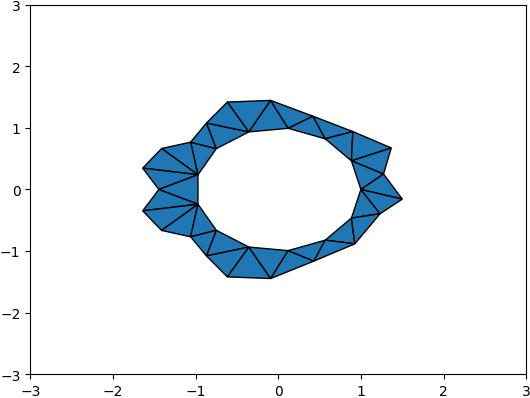
\includegraphics[width=0.70\textwidth]{images/coarse_near_gamma2d.png}
                }
                \vfill
                \item<4->[\checkmark] Build pytential representation
                    of function space
                \vfill
                \item<5->[\checkmark] Build efficient converter between
                    pytential and firedrake representations
                \vfill
                \item<6-> Fully support automatic differentiation
            \end{itemize}
        \vfill
    \item<7-> Evaluation of $\left\langle(i\kappa - \tfrac{\partial}{\partial n})D(u), v\right\rangle_\Sigma$ 
        \begin{itemize}
            \vfill
            \item<8->[\checkmark] \mintinline{python}{LayerPotential} evaluates $D(u)$
                (using pytential under the hood)
            \vfill
            \item<9->[\checkmark] Firedrake evaluates inner product
        \end{itemize}
    \end{itemize}
\end{frame}

%%%%%%%%%%%%%%%%%%%%%%%%                                    %%%%%%%%%%%%%%%%%%%%%%%
%%%%%%%%%%%%%%%%%%%%%%%  Express our problem with firedrake  %%%%%%%%%%%%%%%%%%%%%%%
%%%%%%%%%%%%%%%%%%%%%%%%                                    %%%%%%%%%%%%%%%%%%%%%%%
\begin{frame}[fragile]{Solving the system with Firedrake}
    Extend UFL:
    \[
        a(u, v)
        = \left( \nabla u , \nabla v \right) - \kappa^2 \left( u , v \right)
        - i \kappa \langle u, v \rangle_{\Sigma}
        + \langle \left( i \kappa - \tfrac{\partial}{\partial n} \right) D(u)  v \rangle_\Sigma
    \]
    \only<-2>{
    \visible<2>{
    Will be written as:
    \begin{figure}[ht]
        \begin{center}
            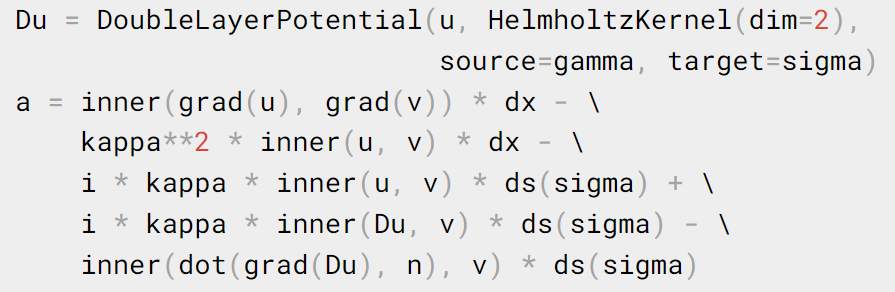
\includegraphics[width=\textwidth]{images/future-code.png}
        \end{center}
    \end{figure}
    }}
    \only<3->{
    Can currently be written as:
    \begin{figure}[ht]
        \begin{center}
            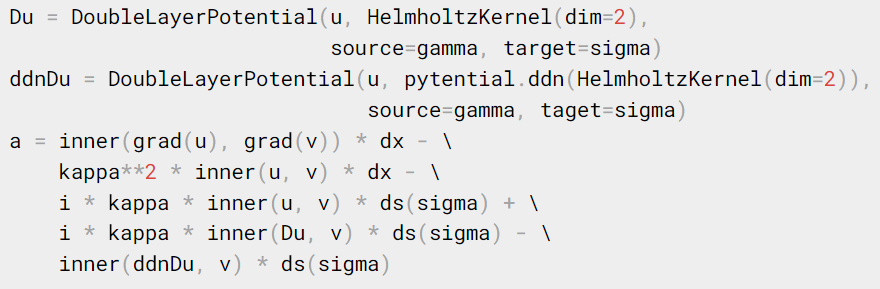
\includegraphics[width=\textwidth]{images/current-code.png}
        \end{center}
    \end{figure}
    }
\end{frame}

\section{Numerical Results}

%%%%%%%%%%%%%%%%%%%%%%%%                %%%%%%%%%%%%%%%%%%%%%%%%
%%%%%%%%%%%%%%%%%%%%%%%  Accuracy plots  %%%%%%%%%%%%%%%%%%%%%%%%
%%%%%%%%%%%%%%%%%%%%%%%%                %%%%%%%%%%%%%%%%%%%%%%%%
\begin{frame}{Numerical results: 2D}
    \visible<2->{
    \begin{figure}[ht]
    \begin{center}
        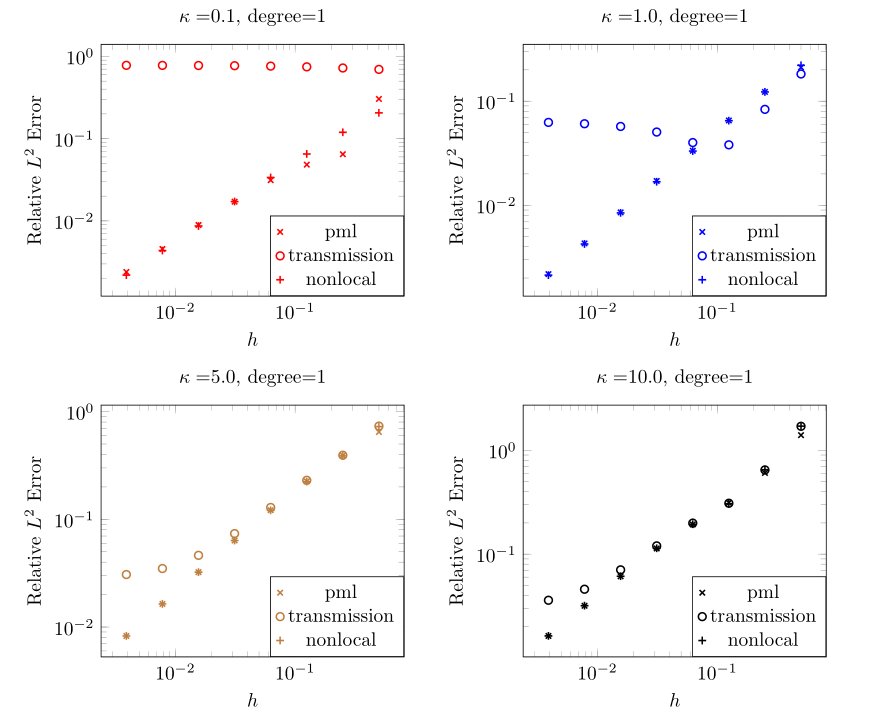
\includegraphics[width=0.8\textwidth]{images/degree-1-accuracy.png}
    \end{center}
    \end{figure}
    }
\end{frame}

%%%%%%%%%%%%%%%%%%%%%%%%                 %%%%%%%%%%%%%%%%%%%%%%%%
%%%%%%%%%%%%%%%%%%%%%%%  Preconditioning  %%%%%%%%%%%%%%%%%%%%%%%%
%%%%%%%%%%%%%%%%%%%%%%%%                 %%%%%%%%%%%%%%%%%%%%%%%%
\begin{frame}{Preconditioning: LU of local part}
    \visible<2->{
    \begin{figure}[ht]
    \begin{center}
        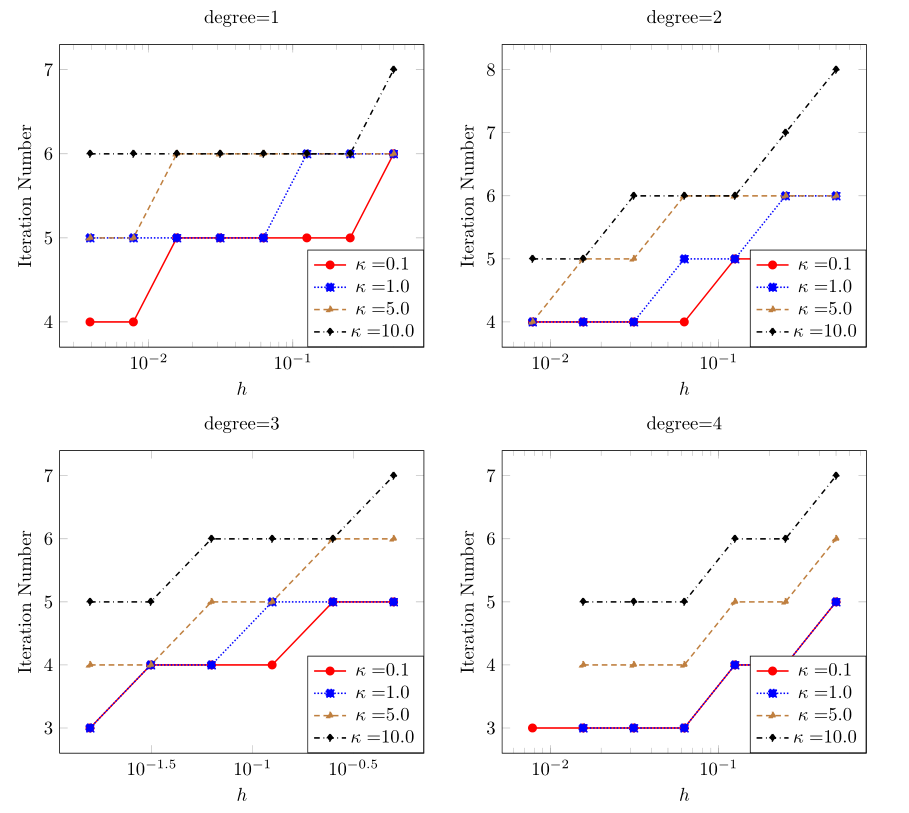
\includegraphics[width=0.75\textwidth]{images/iteration-pc-by-transmission.png}
    \end{center}
    \end{figure}
    }
\end{frame}

%%%%%%%%%%%%%%%%%%%%%%%%       %%%%%%%%%%%%%%%%%%%%%%%%
%%%%%%%%%%%%%%%%%%%%%%%  pyamg  %%%%%%%%%%%%%%%%%%%%%%%%
%%%%%%%%%%%%%%%%%%%%%%%%       %%%%%%%%%%%%%%%%%%%%%%%%
\begin{frame}{Preconditioning: PyAMG}
    \begin{itemize}
        \item If we can find a good preconditioner for the local
            problem, we get a good preconditioner for the nonlocal
            problem
        \vfill
        \item<2->PyAMG:\@ precondition with plane waves
            \begin{figure}[ht]
            \begin{center}
                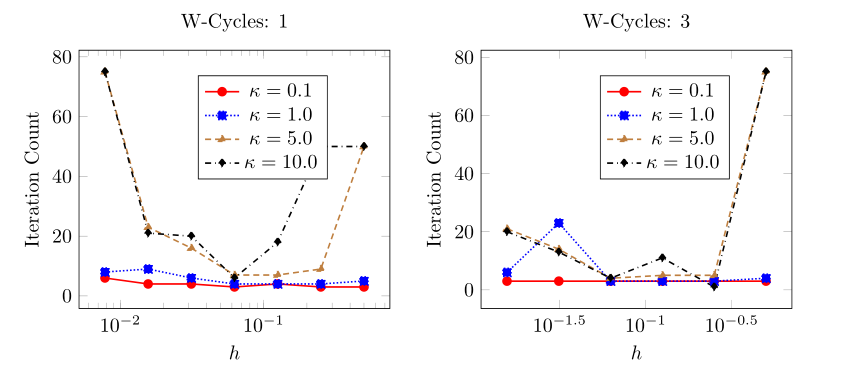
\includegraphics[width=0.8\textwidth]{images/pyamg.png}
            \end{center}
            \end{figure}
    \end{itemize}
\end{frame}

%%%%%%%%%%%%%%%%%%%%%%%%             %%%%%%%%%%%%%%%%%%%%%%%%
%%%%%%%%%%%%%%%%%%%%%%%  Future work  %%%%%%%%%%%%%%%%%%%%%%%%
%%%%%%%%%%%%%%%%%%%%%%%%             %%%%%%%%%%%%%%%%%%%%%%%%
\begin{frame}{Future work}
    \begin{itemize}
        \item<1-> \emph{Coming soon}: automatic differentiation of \mintinline{python}{LayerPotential}s through UFL
        \vfill
        \item<2-> \emph{Coming soon}: \mintinline{python}{VolumePotential}s in UFL
        \vfill
        \item<3-> Leveraging nonlocal UFL to solve more FEM-BEM problems in Firedrake!
            \begin{itemize}
                \item Further investigation into preconditioners
            \end{itemize}
    \end{itemize}
\end{frame}

%
%\begin{frame}[fragile]{Numerical results}
%\begin{figure}
%
%\begin{center}
%    \def \plotaccuracy[#1](#2) % [kappa](color)
%    {
%        \begin{tikzpicture}[scale=0.5]
%        \begin{loglogaxis}[legend style={at={(1.0,0.0)},anchor=south east},
%                           xlabel=$h$,
%                           ylabel=$L^2$ Error,
%                           title={$\kappa=$#1},
%                           filter discard warning=false,
%                           cycle list={
%                               {#2, mark=x}, {#2, mark=o}, {#2, mark=+},
%                           },
%                           scale=0.8]
%            \foreach \method in {pml,transmission,nonlocal} {
               % \addplot+[only marks, thick]
                   % table [x=h,
                          % y expr={\thisrow{kappa}==#1?\thisrow{\method\space lu L2 Error}:nan},
                          % col sep=comma] {data/2d_data.csv};
               % \addlegendentryexpanded{\method};
           % };
       % \end{loglogaxis}
       % \end{tikzpicture}
       % }
   % \begin{tabular}{c c}
   %     \plotaccuracy[0.1](red) & \plotaccuracy[1.0](blue) \\
   %     \plotaccuracy[5.0](brown) & \plotaccuracy[10.0](black) \\
   % \end{tabular}
% \end{center}
%\label{fig:2daccuracy}
%\end{figure}  
%\end{frame}
%
%\begin{frame}{Preconditioning}
%  Flexible GMRES requires right-preconditioning:
%  \[ A \left( P^{-1} \mathbf y \right) = \mathbf b; \ \ \ \mathbf y = P \mathbf x \]%
%  \visible<2->{Our choice of preconditioner\ldots}
%  \visible<3->{\[ P = A^L \] }
%\end{frame}
%
%\begin{frame}{Using LU on $A^L$}
%  \begin{figure}
%\begin{center}
%\begin{tikzpicture}
%    \begin{semilogxaxis}[
%        legend style={at={(1.0,0.0)},anchor=south east},
%        xlabel=$h$,
%        ylabel=Iteration Number,
%        filter discard warning=false,
%        cycle list={%
%            {red, solid, mark=*},
%            {blue, densely dotted, mark=square*},
%            {brown, densely dashed, mark=triangle*},
%            {black, dashdotted, mark=diamond*},
%        }]
%    \foreach \k in {0.1,1.0,5.0,10.0} {
%        \addplot+[thick]
%            table [x=h,
%                   y expr={\thisrow{kappa}==\k?\thisrow{nonlocal lu Iteration Number}:nan},
%                   col sep=comma] {data/2d_data.csv};
%       \addlegendentryexpanded{$\kappa=$\k};
%    };
%    \end{semilogxaxis}
%\end{tikzpicture}
%\end{center}
%\label{fig:luIterationNumber}\end{figure}
%\end{frame}

%\begin{frame}{Scalable: gamg?}
%\begin{figure}
%\begin{center}
%\begin{tikzpicture}[scale=0.5]
%    \begin{semilogxaxis}[
%        legend style={at={(1.0,1.0)},anchor=north east},
%        xlabel=$h$,
%        ylabel=Iteration Number,
%        filter discard warning=false,
%        cycle list={%
%            {red, solid, mark=*},
%            {blue, densely dotted, mark=square*},
%            {brown, densely dashed, mark=triangle*},
%            {black, dashdotted, mark=diamond*},
%        }]
%    \foreach \k in {0.1,1.0} {
%        \addplot+[thick]
%            table [x=h,
%                   y expr={\thisrow{kappa}==\k?\thisrow{nonlocal gamg Iteration Number}:nan},
%                   col sep=comma] {data/2d_data.csv};
%       \addlegendentryexpanded{$\kappa=$\k};
%    };
%    \end{semilogxaxis}
%\end{tikzpicture}
%\end{center}
%\label{fig:gamgIterationNumber}\end{figure}%
%\visible<2->{And explodes for higher $\kappa$.}
%\end{frame}

%% \begin{frame}{What about PyAMG (plane waves)?}
%%   \centering
%%   \includegraphics[width=\textwidth]{foo.pdf}
%% \end{frame}
%\begin{center}
%    \def \plotwcycles[#1]
%    {
%        \begin{tikzpicture}[scale=0.7]
%        \begin{semilogxaxis}[legend style={at={(0.80,0.50)},anchor=south east},
%                             xlabel=$h$,
%                             ylabel=Iteration Count,
%                             title={W-Cycles: #1},
%                             filter discard warning=false,
%                             cycle list={%
%                                {red, solid, mark=*},
%                                {blue, densely dotted, mark=square*},
%                                {brown, densely dashed, mark=triangle*},
%                                {black, dashdotted, mark=diamond*},
%                             },
%                             scale=0.8]
%            \foreach \kappaval in {0.1,1.0,5.0,10.0} {
%                \addplot+[thick]
%                    table [x=h,
%                           discard if not={pyamgmaxiter}{#1},
%                            y expr={\thisrow{kappa}==\kappaval?\thisrow{nonlocal pyamg Iteration Number}:nan},
%                           col sep=comma] {data/pyamg_2d_data.csv};
%                \addlegendentryexpanded{$\kappa=\kappaval$};
%            };
%        \end{semilogxaxis}
%        \end{tikzpicture}
%    }
%    \begin{tabular}{c c}
%        \plotwcycles[1] & \plotwcycles[3]
%    \end{tabular}
% \end{center}


%%%%%%%%%%%%%%%%%%%%%%%%           %%%%%%%%%%%%%%%%%%%%%%%%
%%%%%%%%%%%%%%%%%%%%%%%  Thank you  %%%%%%%%%%%%%%%%%%%%%%%%
%%%%%%%%%%%%%%%%%%%%%%%%           %%%%%%%%%%%%%%%%%%%%%%%%
\begin{frame}[noframenumbering]{Thank you!}
    \begin{center}
        Questions?
    \end{center}
\end{frame}

%%%%%%%%%%%%%%%%%%%%%%%%               %%%%%%%%%%%%%%%%%%%%%%%%
%%%%%%%%%%%%%%%%%%%%%%%  Backup slides  %%%%%%%%%%%%%%%%%%%%%%%%
%%%%%%%%%%%%%%%%%%%%%%%%               %%%%%%%%%%%%%%%%%%%%%%%%
\begin{frame}[noframenumbering]
    \begin{center}
        Backup Slides
    \end{center}
\end{frame}

%%%%%%%%%%%%%%%%%%%%%%%%                     %%%%%%%%%%%%%%%%%%%%%%%%
%%%%%%%%%%%%%%%%%%%%%%%  Theoretical results  %%%%%%%%%%%%%%%%%%%%%%%%
%%%%%%%%%%%%%%%%%%%%%%%%                     %%%%%%%%%%%%%%%%%%%%%%%%
\begin{frame}[noframenumbering]{Theory}
    \begin{itemize}
        \item<2-> $a$ is a bounded bilinear form on $H^1 \times H^1$
        \item<3-> $F$ is a bounded linear functional on $H^1$
        \item<4-> G{\aa}rding inequality. There exist $M$ and an $\alpha > 0$ such that
        \begin{equation*}
            \operatorname{Re}(a(u,u)) + M \left\| u \right\|^2 \geq \alpha \left\| u \right\|_{H^1(\Omega)}^2.
            \end{equation*}
        \item<5-> For $h \leq h_0$, we have optimal-order $H^1$ and $L^2$ error estimaes.
    \end{itemize}
\end{frame}

%%%%%%%%%%%%%%%%%%%%%%%%                      %%%%%%%%%%%%%%%%%%%%%%%%
%%%%%%%%%%%%%%%%%%%%%%%  Extra accuracy plots  %%%%%%%%%%%%%%%%%%%%%%%%
%%%%%%%%%%%%%%%%%%%%%%%%                      %%%%%%%%%%%%%%%%%%%%%%%%
\begin{frame}[noframenumbering]{Numerical results: 2D, degree 2}
    \begin{figure}[ht]
    \begin{center}
        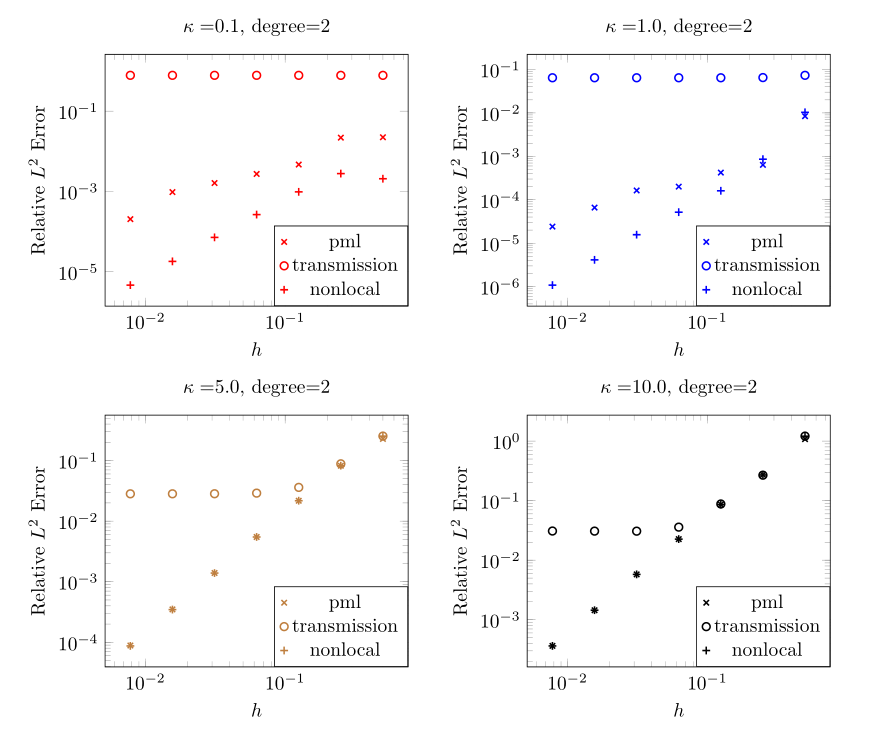
\includegraphics[width=0.8\textwidth]{images/degree-2-accuracy.png}
    \end{center}
    \end{figure}
\end{frame}
\begin{frame}[noframenumbering]{Numerical results: 2D, degree 3}
    \begin{figure}[ht]
    \begin{center}
        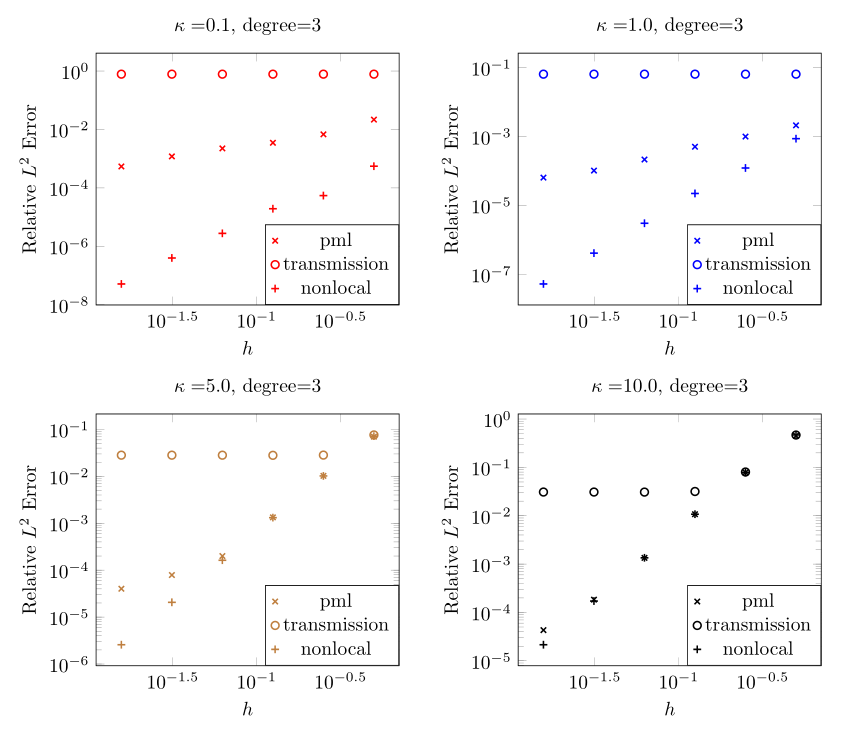
\includegraphics[width=0.8\textwidth]{images/degree-3-accuracy.png}
    \end{center}
    \end{figure}
\end{frame}
\begin{frame}[noframenumbering]{Numerical results: 2D, degree 4}
    \begin{figure}[ht]
    \begin{center}
        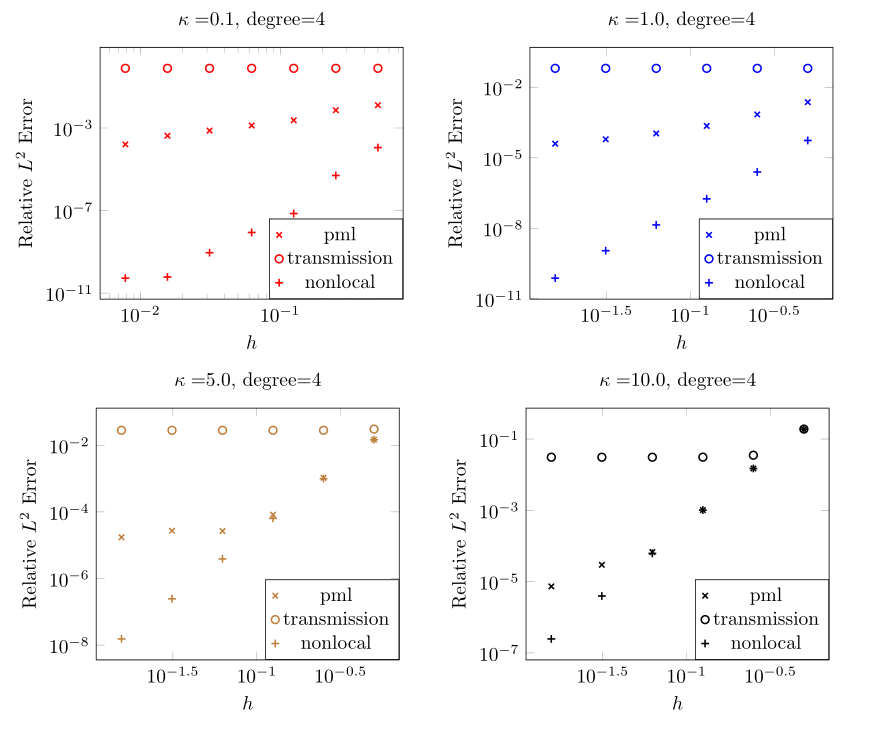
\includegraphics[width=0.8\textwidth]{images/degree-4-accuracy.png}
    \end{center}
    \end{figure}
\end{frame}
\begin{frame}[noframenumbering]{Numerical results: 3D, degree 1}
    \begin{figure}[ht]
    \begin{center}
        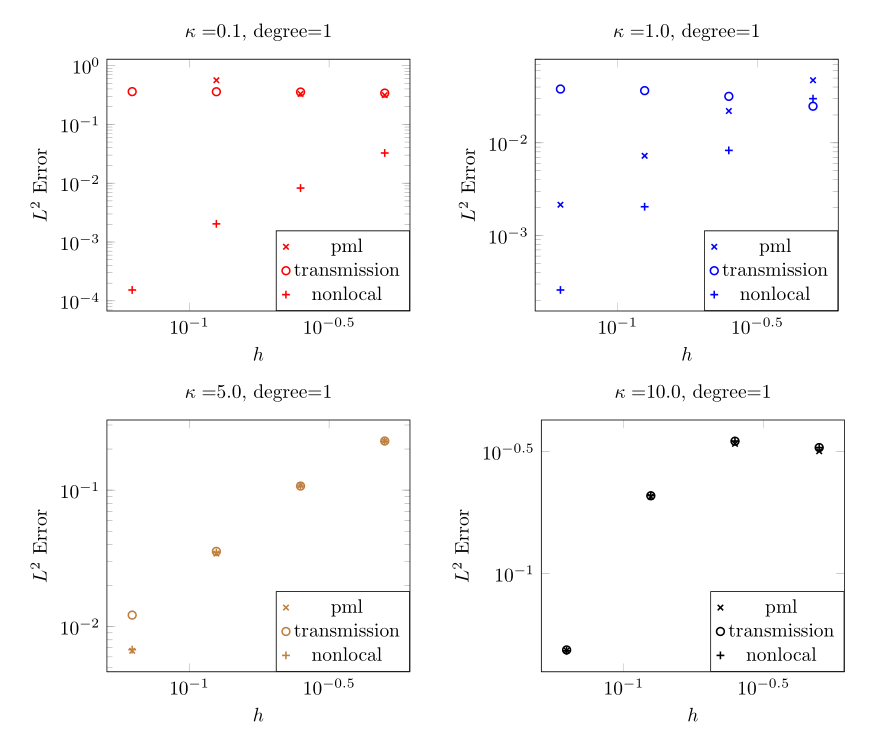
\includegraphics[width=0.8\textwidth]{images/3d-accuracy.png}
    \end{center}
    \end{figure}
\end{frame}

\end{document}
